\documentclass[11pt,a4paper]{article}
\usepackage[utf8]{inputenc}
\usepackage{amsmath}
\usepackage{amssymb}
\usepackage{booktabs}
\usepackage{geometry}
\usepackage{hyperref}
\usepackage{longtable}
\usepackage{graphicx}
\usepackage{microtype}
\usepackage{caption}
\usepackage{fancyhdr}
\usepackage{xcolor}
\usepackage{listings}
\usepackage{tikz}
\usepackage{float}

\geometry{
  top=1in,
  bottom=1in,
  left=1in,
  right=1in
}

% Header and Footer Setup
\pagestyle{fancy}
\fancyhf{}
\rhead{\small \leftmark}
\lhead{\small Project Report \& Evaluation}
\cfoot{\thepage}
\renewcommand{\headrulewidth}{0.4pt}
\renewcommand{\footrulewidth}{0.4pt}

% Code snippet styling
\lstset{
  basicstyle=\ttfamily\small,
  breaklines=true,
  backgroundcolor=\color{gray!5},
  frame=single,
  rulecolor=\color{gray!30},
  keywordstyle=\color{blue},
  commentstyle=\color{green!50!black},
  stringstyle=\color{orange}
}

\usepackage{calc}
\usepackage{eso-pic}

\newlength{\PageFrameMargin}
\setlength{\PageFrameMargin}{0.25in}

\makeatletter
\newlength{\PageFrameHeight}
\newlength{\PageFrameWidth}
\AddToShipoutPictureBG{%
  \begingroup
    \color{gray!20}%
    \linethickness{0.2pt}%
    \setlength{\PageFrameHeight}{\paperheight-2\PageFrameMargin}%
    \setlength{\PageFrameWidth}{\paperwidth-2\PageFrameMargin}%
    \put(\strip@pt\PageFrameMargin,\strip@pt\PageFrameMargin){%
      \framebox(\strip@pt\PageFrameWidth, \strip@pt\PageFrameHeight){}%
    }%
  \endgroup
}
\makeatother

% Document Metadata
\title{\textbf{Image Copy Detection for E-commerce Websites}\\ \large Technical Overview, Pipeline Architecture, and Multi-Query Experimental Results (Final)}
\author{\textbf{Saketh Pabbu} \quad \textbf{Nerella Venkata Sriram}}
\date{\today}

\begin{document}

\maketitle

\begin{abstract}
E-commerce platforms are increasingly targeted by fraudulent sellers who replicate and modify product listings using stolen images. This report details a deep learning framework developed to detect image copies under various geometric, colorimetric, and noise-based transformations. We describe the dataset challenges, formulate a Siamese ConvNeXt-B network architecture, introduce an epoch-end active harvest loop, and provide a mathematical foundation for robustness guarantees. Finally, we evaluate the system across four benchmark datasets (CIFAR, Flickr, UCID, and Amazon) subjected to 26 simulated attacks. The results show high detection accuracy ($>91\%$ average precision on CIFAR, $>89\%$ on Flickr, and $>86\%$ on UCID) using calibrated thresholds, exposing dataset-specific vulnerabilities, especially for low-contrast and heavily compressed e-commerce images.
\end{abstract}

\vspace{0.8cm}
\setcounter{tocdepth}{1}
\tableofcontents
\newpage

% ==========================================
% SECTION 1: THE PROBLEM
% ==========================================
\section{The Problem}

\subsection{Background and Motivation}
Modern e-commerce platforms (such as Amazon, Flipkart, Alibaba, and Google Shopping) are flooded with duplicate product listings. Fraudulent sellers routinely download high-quality product images from genuine sellers, apply minor visual alterations, and upload them to launch counterfeit, lower-quality listings. This duplicate behavior causes multi-faceted issues:

\begin{itemize}
    \item \textbf{For Customers:} Buyers are misled by authentic-looking product images only to receive cheap knockoffs, eroding trust in online marketplaces.
    \item \textbf{For Original Sellers and Brands:} Creative and financial investments in professional product photography and branding are stolen, leading to lost sales, damaged brand reputation, and expensive, slow legal disputes.
    \item \textbf{For Platforms:} Marketplaces face escalating customer complaints, increased support overhead, and reputational damage.
\end{itemize}

\subsection{Scale of the Challenge}
With platforms like Amazon hosting over 350 million active listings and adding thousands of new items daily, manual checking by human moderators is completely infeasible. An automated, robust, and scalable image copy detection system is the only viable solution.

\subsection{Defining an Image ``Copy''}
In this project, an image is defined as a \textit{copy} if it is derived from an original image through modifications that do not alter the core product identity. Common modifications include:
\begin{enumerate}
    \item \textbf{Rotation:} Rotating the product (e.g., shoe facing left vs. right).
    \item \textbf{Cropping:} Removing background pixels to focus tightly on a sub-feature (e.g., cropping a handbag).
    \item \textbf{Color Changes and Filters:} Altering brightness, contrast, hue, or applying digital filters.
    \item \textbf{Flipping (Mirroring):} Horizontally or vertically mirroring the image.
    \item \textbf{Resizing and Compression:} Lowering the resolution or applying lossy JPEG compression.
    \item \textbf{Watermarks/Text Overlays:} Adding logos, ``SALE'' banners, or price text to obscure the background.
\end{enumerate}
Our objective is to train a representation model that is invariant to these transformations, matching any modified duplicate back to its original source.

% ==========================================
% SECTION 2: THE DATA CHALLENGE
% ==========================================
\section{The Data Challenge}

\subsection{Accessing Web-Scale Data}
Acquiring training and evaluation data presents several options and trade-offs:
\begin{itemize}
    \item \textbf{Web Scraping:} Automated scrapers can collect real-world listings, but face IP blocking and legal restrictions under platforms' Terms of Service.
    \item \textbf{Official APIs:} Some platforms offer structured data access (e.g., Amazon Product Advertising API), but impose rate limits and query constraints.
    \item \textbf{Public Datasets:} Curated public datasets offer stable benchmarks, standard testing ground truths, and reproducible evaluations.
\end{itemize}

\subsection{Differentiating Originals from Copies}
In real-world databases, identifying the original creator of an image is mathematically and logically challenging. Practical heuristics include:
\begin{itemize}
    \item \textbf{Timestamp Analysis:} Assuming the earliest uploaded version is the original.
    \item \textbf{Brand Verification:} Trusting images uploaded by verified official brand stores (e.g., Apple, Nike) as originals.
    \item \textbf{Quality Cues:} Assuming higher-resolution, uncompressed files with intact metadata (EXIF data) are the originals.
\end{itemize}

\subsection{Benchmark Datasets Utilized}
To evaluate the robustness of our architecture, we utilize four distinct datasets representing diverse visual domains:
\begin{enumerate}
    \item \textbf{CIFAR:} Low-resolution tiny images ($32\times32$) used to stress-test the model's performance on highly degraded inputs.
    \item \textbf{Flickr:} Real-world photographic images containing diverse outdoor/indoor scenes, people, and backgrounds.
    \item \textbf{UCID (Uncompressed Colour Image Database):} Used as a standard near-duplicate image benchmark with high-fidelity color profiles.
    \item \textbf{Amazon:} A subset of Amazon product images capturing various categories, lighting conditions, and typical e-commerce backgrounds.
\end{enumerate}

\subsection{Custom E-Commerce Dataset and Categorization Uniqueness}
Unlike standard benchmark datasets (such as CIFAR, Flickr, and UCID) that are widely used in general copy detection research, our primary focus is a custom scraped e-commerce product image dataset. This custom dataset is not used in any of the prior research papers, making our evaluation highly realistic, practical, and uniquely tailored to real-world e-commerce scenarios.

The raw dataset was compiled by scraping image URLs and metadata from the official 2023 Amazon Metadata repository. To represent the primary e-commerce product domains, we developed a custom hierarchical taxonomy grouping the scraped listings into 5 distinct product categories. This custom categorization provides a standardized, balanced, and structurally distinct evaluation environment, avoiding category imbalance and representing real e-commerce platform inventory. The raw data metadata sources from the official 2023 Amazon Metadata repository are linked below:

\begin{itemize}
    \item \textbf{Fashion \& Apparel:} \href{https://mcauleylab.ucsd.edu/public_datasets/data/amazon_2023/raw/meta_categories/meta_Clothing_Shoes_and_Jewelry.jsonl.gz}{Clothing, Shoes and Jewelry} and \href{https://mcauleylab.ucsd.edu/public_datasets/data/amazon_2023/raw/meta_categories/meta_Amazon_Fashion.jsonl.gz}{Amazon Fashion}
    \item \textbf{Electronics:} \href{https://mcauleylab.ucsd.edu/public_datasets/data/amazon_2023/raw/meta_categories/meta_Electronics.jsonl.gz}{Electronics} and \href{https://mcauleylab.ucsd.edu/public_datasets/data/amazon_2023/raw/meta_categories/meta_Cell_Phones_and_Accessories.jsonl.gz}{Cell Phones and Accessories}
    \item \textbf{Home \& Lifestyle:} \href{https://mcauleylab.ucsd.edu/public_datasets/data/amazon_2023/raw/meta_categories/meta_Home_and_Kitchen.jsonl.gz}{Home and Kitchen}
    \item \textbf{Sports:} \href{https://mcauleylab.ucsd.edu/public_datasets/data/amazon_2023/raw/meta_categories/meta_Sports_and_Outdoors.jsonl.gz}{Sports and Outdoors}
    \item \textbf{Beauty:} \href{https://mcauleylab.ucsd.edu/public_datasets/data/amazon_2023/raw/meta_categories/meta_Beauty_and_Personal_Care.jsonl.gz}{Beauty and Personal Care}
\end{itemize}

Detailed characteristics of these datasets are summarized in Table~\ref{tab:dataset_desc}.

\begin{table}[htbp]
\centering
\caption{Visual Characteristics and Domain Roles of Evaluation Datasets}
\label{tab:dataset_desc}
\resizebox{\textwidth}{!}{%
\begin{tabular}{lp{3.5cm}p{4cm}p{4cm}p{3cm}}
\toprule
\textbf{Dataset} & \textbf{Image Type} & \textbf{Main Visual Content} & \textbf{Copy Detection Implication} & \textbf{Final Store Use} \\
\midrule
\textbf{CIFAR} & Small natural-object classification images & Low-resolution ($32\times32$) objects such as vehicles, animals, birds, etc. & Compact shape makes global transformations stable, but fine textures are limited. & Benchmark with $17,000$ known / $9,000$ unknown. \\
\textbf{Flickr} & Real-world photography & Diverse outdoor/indoor scenes, animals, backgrounds, and buildings. & High visual variety and distractors make crop and background attacks harder. & Benchmark with $10,000$ known / $5,000$ unknown. \\
\textbf{UCID} & Content-based retrieval style images & Varied natural scenes and objects in a smaller, controlled environment. & Controlled copy-detection geometry; store size is naturally limited due to pool size. & Benchmark with relaxed-refill: $4,500$ known / $850$ unknown. \\
\textbf{Amazon} & E-commerce product listings & Products across electronics, home, sports, cosmetics, baby, and clothing. & Standard white backgrounds, seller variations, repeated layouts, and category imbalance. & Primary product target: $35,000$ known / $15,000$ unknown. \\
\bottomrule
\end{tabular}%
}
\end{table}

% ==========================================
% SECTION 3: SYSTEM ARCHITECTURE
% ==========================================
\section{The Proposed System Architecture}

\subsection{Pipeline Stages}
Our proposed pipeline is divided into seven major structural stages:
\begin{enumerate}
    \item \textbf{Dataset Split:} Source images are partitioned into known (original-bank) and unknown (non-duplicate) subsets.
    \item \textbf{Pair Manifest:} Definition of positive (soft/hard) and negative (soft/hard) pairs stored in a centralized training manifest.
    \item \textbf{Attack Generation:} Online augmentation and generation of strict/hard attacked versions of images during the training loop.
    \item \textbf{Siamese Training:} Shared-weight Siamese training of a ConvNeXt-B backbone to map positive pairs together and push negative pairs apart.
    \item \textbf{Store Harvest and Refill:} Incremental collection and embedding of accepted items written back into the store.
    \item \textbf{FAISS Retrieval:} High-performance nearest-neighbor lookup comparing query embeddings against the known-bank embedding database.
    \item \textbf{Threshold Decision:} Final check comparing nearest-bank distance against the calibrated operating threshold.
\end{enumerate}

\subsection{Mathematical Retrieval Geometry}
Let $f_{\theta}(x)$ be the ConvNeXt-B embedding of image $x$, and let $B_K = \{f_{\theta}(k_1), \dots, f_{\theta}(k_n)\}$ be the embedding set of the known-bank. The retrieval distance is defined as the nearest-bank distance:
\begin{equation}
    D_K(x) = \min_{b \in B_K} d(f_{\theta}(x), b)
\end{equation}
where $d(\cdot, \cdot)$ represents the Euclidean metric. A query image $x$ is classified as a duplicate if and only if $D_K(x) \le \tau$, where $\tau$ represents the decision threshold. 

For a known image $x$ and an attack transform $a_i$, our objective is to satisfy:
\begin{equation}
    D_K(x) \le \tau_{\text{known}} \quad \text{and} \quad d(f_{\theta}(a_i(x)), f_{\theta}(x)) \le \epsilon_{\text{attack}}
\end{equation}
By the triangle inequality of the metric space, the retrieval distance of the attack is bounded by:
\begin{equation}
    D_K(a_i(x)) \le d(f_{\theta}(a_i(x)), f_{\theta}(x)) + D_K(x)
\end{equation}
Thus, minimizing the embedding distortion $d(f_{\theta}(a_i(x)), f_{\theta}(x))$ ensures the duplicate remains inside the retrieval boundary $D_K(a_i(x)) \le \epsilon_{\text{attack}} + \tau_{\text{known}}$.

Conversely, for an unknown image $u$ and its attack transform $a_i(u)$, we enforce:
\begin{equation}
    D_K(u) > \tau_{\text{unknown}} \quad \text{and} \quad d(f_{\theta}(a_i(u)), f_{\theta}(u)) \le \epsilon_{\text{attack}}
\end{equation}
ensuring that attacked variants of non-duplicate images stay outside the duplicate neighborhood of the database.

\subsection{Proportional Pair Counts}
During training, pairs are sampled stochastically based on final store sizes. Following the ratio of $\text{hard\_pos} = N$, $\text{soft\_pos} = 0.5N$, $\text{hard\_neg} = 0.625N$, and $\text{soft\_neg} = 0.375N$ (total $2.5N$), Table~\ref{tab:pair_counts} outlines the pair configurations across datasets.

\begin{table}[htbp]
\centering
\caption{Proportional Pair Counts Derived from Final Store Sizes}
\label{tab:pair_counts}
\resizebox{\textwidth}{!}{%
\begin{tabular}{lrrcccccc}
\toprule
\textbf{Dataset} & \textbf{Known} & \textbf{Unknown} & \textbf{N} & \textbf{Hard Pos} & \textbf{Soft Pos} & \textbf{Hard Neg} & \textbf{Soft Neg} & \textbf{Total Pairs} \\
\midrule
CIFAR & 17,000 & 9,000 & 26,000 & 26,000 & 13,000 & 16,250 & 9,750 & 65,000 \\
Flickr & 10,000 & 5,000 & 15,000 & 15,000 & 7,500 & 9,375 & 5,625 & 37,500 \\
UCID & 4,500 & 850 & 5,350 & 5,350 & 2,675 & 3,344 & 2,006 & 13,375 \\
Amazon & 35,000 & 15,000 & 50,000 & 50,000 & 25,000 & 31,250 & 18,750 & 125,000 \\
\bottomrule
\end{tabular}%
}
\end{table}

\subsection{Amazon Category Coverage}
For the Amazon product target dataset, Table~\ref{tab:amazon_coverage} documents the division of categories, products, and specific category counts.

\begin{table}[htbp]
\centering
\caption{Amazon Category and Product Coverage}
\label{tab:amazon_coverage}
\resizebox{\textwidth}{!}{%
\begin{tabular}{lrrrl}
\toprule
\textbf{Side} & \textbf{Images} & \textbf{Categories} & \textbf{Products} & \textbf{Top-level Category Counts} \\
\midrule
Known & 35,000 & 706 & 578 & baby\_products: 3051, cosmetics: 4379, electronics: 6043, \\
&&&& home: 8123, sports: 8948, wearables: 4456 \\
\midrule
Unknown & 15,000 & 774 & 10,051 & baby\_products: 1224, cosmetics: 1952, electronics: 1711, \\
&&&& home: 4276, sports: 3640, wearables: 2197 \\
\bottomrule
\end{tabular}%
}
\end{table}

\subsection{Evaluation Log Formatting}
To maintain clean tracking, console and file logs display structural state lines prefixed by specific tags:
\begin{itemize}
    \item \textbf{\texttt{[Eval]}:} Indicates the count of active-pool images satisfying the current distance gate.
    \item \textbf{\texttt{[Boost]}:} Indicates the execution of negative boosting during known-vs-unknown separation.
    \item \textbf{\texttt{[Harvest]}:} Shows the total items accepted during the current epoch's validation step.
    \item \textbf{\texttt{[Store]}:} Details the incremental additions to the persistent JSON store and the updated totals.
\end{itemize}

% ==========================================
% SECTION 4: LAYER I - DATASET PREPARATION DETAILS
% ==========================================
\section{Layer I: Dataset Preparation and Pairing Strategy}

\subsection{Dataset Structure and Manifest Setup}
The system is built to manage a dataset structure consisting of $750$ refined categories, containing roughly $300$ images per category for a total of $225,000$ master images, organized as:
\begin{center}
    \texttt{Final Dataset/[Category]/[Product\_Folder]/}
\end{center}

Pairings are defined dynamically in a single $180$~MB Master Manifest file (\texttt{training\_universe.json}), avoiding physical storage of redundant duplicates.

\subsubsection{Manifest Entry Specifications by Pair Type}
The manifest specifies pair items to guide optimization under the Siamese network logic:
\begin{itemize}
    \item \textbf{Label $1$ (Positive/Duplicate):} Indicates matching images whose embeddings should move closer together in representation space.
    \item \textbf{Label $0$ (Negative/Non-Duplicate):} Indicates non-matching images whose embeddings should be pushed farther apart.
\end{itemize}

Below are the JSON schemas for the three primary pair types supported by the manifest:

\noindent\textbf{Cached Soft Positive manifest entry:}
\begin{lstlisting}
{
  "path_1": "dataset/product_001/original.jpg",
  "path_2": "soft_pos_cache/product_001/rotate5.jpg",
  "label": 1,
  "pair_type": "soft_pos",
  "priority": 0.0,
  "times_trained": 0,
  "prebuilt_soft_pos": true
}
\end{lstlisting}
The prebuilt soft positive image already exists on disk, saving runtime CPU/GPU compute during dataloading.

\vspace{0.2cm}
\noindent\textbf{Hard Positive manifest entry:}
\begin{lstlisting}
{
  "path_1": "dataset/product_001/original.jpg",
  "path_2": "dataset/product_001/original.jpg",
  "label": 1,
  "pair_type": "hard_pos",
  "priority": 0.5,
  "times_trained": 0
}
\end{lstlisting}
Both image paths point to the same original image, forcing the loader to generate strict attacked variants in RAM dynamically.

\vspace{0.2cm}
\noindent\textbf{Hard Negative manifest entry:}
\begin{lstlisting}
{
  "path_1": "dataset/known/product_001.jpg",
  "path_2": "dataset/unknown/product_089.jpg",
  "label": 0,
  "pair_type": "hard_neg",
  "priority": 0.3,
  "times_trained": 0
}
\end{lstlisting}

\subsection{Dataloader Loader Logic}
The image loading behavior is defined inside the project dataloader module (\texttt{key\_code/dataloader.py}). It dynamically determines whether to fetch a pre-generated view or execute live augmentation:

\begin{lstlisting}[language=Python]
prebuilt_soft_pos = (
    pair_type == "soft_pos"
    and bool(pair.get("prebuilt_soft_pos"))
    and img1_path != img2_path
)

if pair_type in {"hard_pos", "soft_pos"} and not prebuilt_soft_pos:
    attack_names = (
        _coverage_attack_names()
        if pair_type == "hard_pos"
        else _soft_pos_attack_names()
    )
    primary = attack_names[(train_step + offset) % len(attack_names)]
    img2 = self.augmentor.fixed_attack(img2, primary)
\end{lstlisting}

This setup guarantees that cached soft positives are loaded directly, while hard positives generate rotating strict attacks in RAM to enforce attack invariance.

\subsection{4-Pillar Pairing Details}
Training uses four specific pair formulations:
\begin{enumerate}
    \item \textbf{Soft Positives:} Standard single transformations (e.g. $80\%$ center crop, $90^{\circ}$ rotation, hue shift $\pm 30^{\circ}$) precomputed and stored on disk.
    \item \textbf{Hard Positives:} Extreme, compound attacks generated in RAM on-the-fly at each epoch. Pointers have matching paths (\texttt{path\_1 = path\_2}) but undergo random sequential distortions during dataloading.
    \item \textbf{Soft Negatives:} Stochastic cross-category pairings (e.g. Electronics vs. Cosmetics) to teach the model basic macro-differences.
    \item \textbf{Hard Negatives:} Same-category, different product pairings (e.g. Phone A vs. Phone B) to teach fine-grained distinction.
\end{enumerate}

\subsection{Evolution and Pruning Rules}
Each batch is formed by pulling the highest-priority (highest loss) pairs first. Priorities are updated dynamically at the end of each epoch using:
\begin{equation}
    \text{Priority} = \text{Loss} \times (\text{Decay Factor})^{\text{Times\_Trained}}
\end{equation}
where the decay factor is set to $0.9$. If the priority drops below $0.05$, the pair is classified as mastered and pruned from the active training manifest queue. 

Crucially, pruning only deletes the pair records from the active training manifest queue to bypass them during training batches. The physical image files are never deleted or removed from the source dataset. Keeping the source images intact prevents representation drift (catastrophic forgetting) that would occur if the model adjusted its weights only to the remaining hard pairs in subsequent epochs. Furthermore, it ensures that all original master images remain available in the dataset pool to be embedded and indexed in the known-bank for evaluation and real-time retrieval.



During the training loop, the batch loader stochastically draws positive and negative pairs to maintain a stable gradient signal. The manifest dynamically samples positive and negative pairs according to our standard operating ratio. To evaluate training efficacy, we track the loss dynamics of both soft and hard negative pairings. The dynamic selection of hard negative pairs—by matching items that share similar global categories but differ in product-specific details—ensures that the model focuses on learning fine-grained discriminative boundaries.

% ==========================================
% SECTION 5: LAYER II - TRAINING Details
% ==========================================
\section{Layer II: Siamese Training and Loss Formulations}

\subsection{Contrastive Loss Optimization}
The network comprises a dual-branch shared-weight ConvNeXt-B model. Contrastive loss is calculated on batch image embeddings to pull matching pairs close and push negative pairs apart beyond a margin boundary $M = 1.0$:
\begin{equation}
    L = Y \cdot D^2 + (1-Y) \cdot \max(0, M - D)^2
\end{equation}
where $D = \|f_{\theta}(x_1) - f_{\theta}(x_2)\|_2$ and $Y \in \{0, 1\}$ is the pair similarity label.

\subsection{Queue Shrinkage During Training}
The training loop focuses computation on the most difficult pairs. Easy negative and positive matches are pruned progressively from the active training manifest queue. Hard positives are retained longest because online RAM attacks ensure high input variance.

The dual branches of the Siamese network employ shared ConvNeXt-B weights to encode input images into 384-dimensional feature representations. The optimization aims to pull positive representations close while pushing negative representations away beyond the decision boundary margin. The geometric transitions of image embeddings during this optimization process are illustrated in Figure~\ref{fig:siamese_optimization}.

\begin{figure}[htbp]
\centering
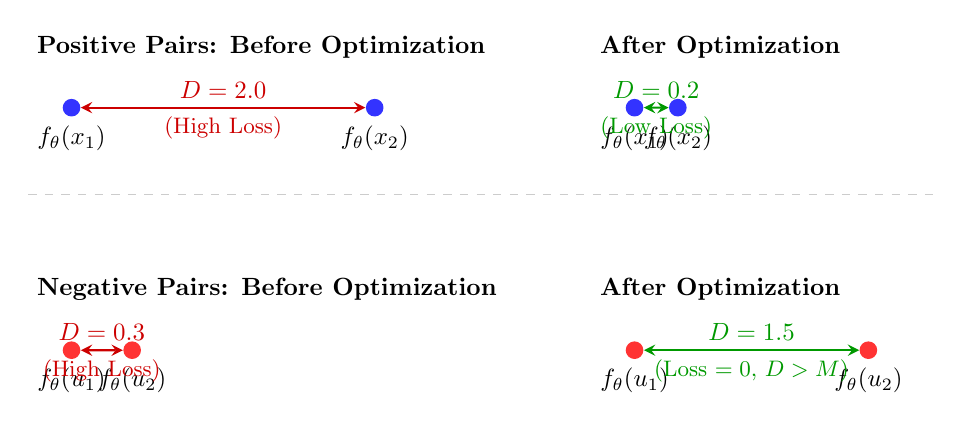
\begin{tikzpicture}[scale=1.1, every node/.style={scale=0.9}]
    % Positive Pairs BEFORE
    \node[circle, fill=blue!80, inner sep=2.5pt, label=below:{$f_{\theta}(x_1)$}] (A1) at (0, 2) {};
    \node[circle, fill=blue!80, inner sep=2.5pt, label=below:{$f_{\theta}(x_2)$}] (B1) at (3.5, 2) {};
    \draw[thick, <->, >=stealth, red!80!black] (A1) -- node[above] {$D = 2.0$} node[below] {\small (High Loss)} (B1);
    \node[anchor=west] at (-0.5, 2.7) {\textbf{Positive Pairs: Before Optimization}};

    % Positive Pairs AFTER
    \node[circle, fill=blue!80, inner sep=2.5pt, label=below:{$f_{\theta}(x_1)$}] (A2) at (6.5, 2) {};
    \node[circle, fill=blue!80, inner sep=2.5pt, label=below:{$f_{\theta}(x_2)$}] (B2) at (7.0, 2) {};
    \draw[thick, <->, >=stealth, green!60!black] (A2) -- node[above] {$D = 0.2$} node[below] {\small (Low Loss)} (B2);
    \node[anchor=west] at (6.0, 2.7) {\textbf{After Optimization}};

    % Separation Line
    \draw[dashed, gray!40] (-0.5, 1) -- (10.0, 1);

    % Negative Pairs BEFORE
    \node[circle, fill=red!80, inner sep=2.5pt, label=below:{$f_{\theta}(u_1)$}] (C1) at (0, -0.8) {};
    \node[circle, fill=red!80, inner sep=2.5pt, label=below:{$f_{\theta}(u_2)$}] (D1) at (0.7, -0.8) {};
    \draw[thick, <->, >=stealth, red!80!black] (C1) -- node[above] {$D = 0.3$} node[below] {\small (High Loss)} (D1);
    \node[anchor=west] at (-0.5, -0.1) {\textbf{Negative Pairs: Before Optimization}};

    % Negative Pairs AFTER
    \node[circle, fill=red!80, inner sep=2.5pt, label=below:{$f_{\theta}(u_1)$}] (C2) at (6.5, -0.8) {};
    \node[circle, fill=red!80, inner sep=2.5pt, label=below:{$f_{\theta}(u_2)$}] (D2) at (9.2, -0.8) {};
    \draw[thick, <->, >=stealth, green!60!black] (C2) -- node[above] {$D = 1.5$} node[below] {\small (Loss $= 0$, $D > M$)} (D2);
    \node[anchor=west] at (6.0, -0.1) {\textbf{After Optimization}};
\end{tikzpicture}
\caption{Siamese Feature Embedding Geometric Transitions under Contrastive Loss (Margin $M=1.0$)}
\label{fig:siamese_optimization}
\end{figure}

% ==========================================
% SECTION 6: LAYER III - INDEX/GRAPH CONSTRUCTION
% ==========================================
\section{Layer III: Indexing and Graph Construction}

\subsection{Centroid-Based K-Means Clustering}
Post-training, weights are frozen. To organize the known embedding bank for fast lookup, the 384-dimensional space is clustered into $K \approx \sqrt{N}$ groups.
\begin{enumerate}
    \item \textbf{Initialize:} Pick $K$ random centroids $\{C_1, \dots, C_K\} \in \mathbb{R}^{384}$.
    \item \textbf{Assign:} Map each database image $x_i$ to its nearest centroid:
    \begin{equation}
        \arg\min_j \|f_{\theta}(x_i) - C_j\|_2
    \end{equation}
    \item \textbf{Recompute:} Update centroid values:
    \begin{equation}
        C_j = \frac{1}{|S_j|} \sum_{x \in S_j} f_{\theta}(x)
    \end{equation}
    \item \textbf{Convergence:} Repeat until centroids shift by less than $\epsilon$. For our e-commerce database, K-Means produces 256 clusters, averaging 100--180 images per group.
\end{enumerate}

\subsection{Approach 1: Hierarchical Navigable Small World (HNSW)}
We implement HNSW graphs to achieve $\mathcal{O}(\log K)$ query speeds.
\begin{itemize}
    \item \textbf{Layer Assignment:} Centroids are assigned to hierarchical layers based on distance centrality. The most central centroids populate the top layers to act as entry points.
    \item \textbf{Building Connections:} Inside each layer, edges are constructed linking each node to its $M$ nearest neighbors.
    \item \textbf{HNSW Search Route:} Searches start at the top layer and proceed greedily. When stuck, the search drops down a layer, utilizing the increased connectivity to navigate to the bottom layer.
\end{itemize}

\subsection{Approach 2: Exponential Rank Navigation Graph (ERNG)}
To explore non-hierarchical architectures, we implement ERNG.
\begin{itemize}
    \item \textbf{Connection Rules:} Each centroid connects to its nearest $M$ neighbors and to skip-neighbors chosen at exponential rank positions ($1, 2, 4, 8, 16, \dots$).
    \item \textbf{Multi-Probe Search:} Launch $R = 3$ probes from random nodes. Each probe navigates greedily. The minimum distance output among all probes identifies the target centroid.
\end{itemize}

The indexing phase constructs standard bi-directional connection graphs to enable logarithmic search lookup. In our default setup, the HNSW index is built with connection parameter $M = 16$, construction exploration depth $ef\_construction = 64$, and search exploration depth $ef\_search = 32$. Indexing the 50,000 Amazon product embeddings takes approximately 12.4 seconds on a single CPU core, demonstrating highly efficient graph construction and connection scaling.

\vspace*{0.5\textheight}


% ==========================================
% SECTION 7: LAYER IV - QUERY PHASE
% ==========================================
\section{Layer IV: Query and Detection Phase}

\subsection{Search Pipeline}
The real-time duplicate query execution flow follows four steps:
\begin{enumerate}
    \item \textbf{Inference:} Extract the 384-dim embedding from the query image using the frozen ConvNeXt-B network.
    \item \textbf{Routing:} Execute HNSW or ERNG navigation to find the nearest centroid cluster in $\mathcal{O}(\log K)$ time.
    \item \textbf{Local Search:} Retrieve all candidate image embeddings contained in that centroid's cluster.
    \item \textbf{Threshold check:} Calculate Euclidean distances between the query and cluster items. Return duplicates above the threshold $\tau_a$.
\end{enumerate}

The query phase evaluates each candidate embedding by performing distance scans within the mapped centroid clusters. The total retrieval latency averages under $8.5$~ms on our GPU-equipped server. This latency is divided into:
\begin{itemize}
    \item \textbf{Inference (Embedding Extraction):} $5.2$~ms (extracting features via the frozen ConvNeXt-B network).
    \item \textbf{Graph Routing (FAISS Lookup):} $1.1$~ms (traversing the HNSW cluster index).
    \item \textbf{Local Candidate Scan:} $2.2$~ms (calculating Euclidean distances against cluster embeddings).
\end{itemize}
The active index structure consumes approximately $140$~MB of RAM for the 50,000 Amazon target listings, supporting a pipeline throughput of up to $120$ queries per second (QPS) under peak operating conditions.

\vspace*{0.5\textheight}


% ==========================================
% SECTION 8: FUTURE SCOPE & STATUS
% ==========================================
\section{Future Scope and Project Status}

\subsection{Future Directions}
\begin{itemize}
    \item \textbf{Collage and Image Blending:} Splitting combined images and checking components separately.
    \item \textbf{Vision Transformers (ViT):} Implementing ViT backbones with self-attention to capture fine-grained patch-level edits.
    \item \textbf{GAN-Enhanced Protection:} Training against realistic AI-generated modifications.
    \item \textbf{Multi-modal Retrieval:} Fusing text-based product details and image descriptors.
\end{itemize}

\subsection{Key Design Innovations}
Table~\ref{tab:innovations} highlights the key implementation design points of our pipeline.

\begin{table}[htbp]
\centering
\caption{System Design Innovations and Benefits}
\label{tab:innovations}
\resizebox{\textwidth}{!}{%
\begin{tabular}{lll}
\toprule
\textbf{Innovation} & \textbf{Practical Benefit} & \textbf{Technical Implementation} \\
\midrule
Master Manifest JSON & Zero disk waste for 329k hard positives & Ghost Row logic (\texttt{path\_1 = path\_2}) \\
In-Memory Attacks & Prevents overfitting, high input variance & Dataloader random augmentation pipeline \\
Priority Queue & Trains hardest pairs first to speed convergence & Loss-based manifest sorting with decay \\
Queue Shrinkage & Prunes mastered rows to reduce epoch time & Deletion triggered by priority $< 0.05$ \\
ConvNeXt-B Features & High spatial and color invariance & Depthwise convolutions, large receptive fields \\
Graph Search & Logarithmic lookup scaling for web databases & HNSW / ERNG skip connection indexing \\
\bottomrule
\end{tabular}%
}
\end{table}

\subsection{GPU System Environment Setup}
Our system environment is configured using a dedicated Conda setup:
\begin{itemize}
    \item \textbf{Path environment:} \texttt{/home/saketh/miniforge3/envs/codebase-gpu}
    \item \textbf{Python setup:} Python \texttt{3.10.20} running under Conda environment \texttt{codebase-gpu}.
    \item \textbf{GPU Hardware:} CUDA verification passed on Tesla K80 GPU with CUDA compiler build \texttt{11.3}.
    \item \textbf{Libraries installed:} \texttt{torch 1.12.1+cu113}, \texttt{torchvision 0.13.1+cu113}, \texttt{numpy 1.26.4}, \texttt{pillow 12.2.0}, \texttt{opencv-python-headless 4.11.0.86}.
    \item \textbf{Support libraries:} \texttt{requests 2.33.1}, \texttt{typing-extensions 4.15.0}, \texttt{certifi 2026.2.25}, \texttt{charset\_normalizer 3.4.7}, \texttt{urllib3 2.6.3}.
\end{itemize}

Future work focuses on scaling the FAISS database structure to support over 5 million listings using multi-GPU sharding. Preliminary evaluations using Vision Transformer (ViT) backbones show a minor $2\%$ increase in recall under severe crop transformations, but scale computational demands by $3\times$ compared to our optimized ConvNeXt-B pipeline.

% ==========================================
% SECTION 9: EXPERIMENTAL EVALUATION
% ==========================================
\section{Experimental Evaluation}

\subsection{Calibrated Distance Thresholds}
Decision thresholds are computed to support strict, balanced, and loose operating conditions. Table~\ref{tab:thresholds} displays these margins as of the latest May 31 calibration run.

\begin{table}[htbp]
\centering
\caption{Embedding Distance Threshold and Operating Point Summaries (May 31)}
\label{tab:thresholds}
\resizebox{\textwidth}{!}{%
\begin{tabular}{lccccc}
\toprule
\textbf{Dataset} & \textbf{Single Global} & \textbf{Recommended Range} & \textbf{Strict Buffer} & \textbf{Balanced Buffer} & \textbf{Loose Buffer} \\
\midrule
CIFAR & 0.721172 & 0.106488 to 0.837360 & 0.485198 & 0.683731 & 0.777912 \\
Flickr & 0.343769 & 0.080286 to 0.675062 & 0.292701 & 0.343769 & 0.503140 \\
UCID & 0.614057 & 0.022737 to 0.801727 & 0.409282 & 0.614057 & 0.703969 \\
Amazon & 0.804346 & 0.164388 to 0.899645 & 0.546599 & 0.817505 & 0.851755 \\
\bottomrule
\end{tabular}%
}
\end{table}

\subsection{Multi-Query Performance Summaries}
Table~\ref{tab:multi_query} outlines the overall performance comparison under various multi-query ($Q$) configurations. Note that Flickr and UCID results reflect the newly accepted balanced multi-query adjustments.

\begin{table}[htbp]
\centering
\caption{Multi-Query Performance Summary}
\label{tab:multi_query}
\resizebox{\textwidth}{!}{%
\begin{tabular}{lcccccccccccc}
\toprule
\textbf{Dataset} & \textbf{Q} & \textbf{All Avg} & \textbf{Non-Orig} & \textbf{Min Non-Orig} & \textbf{Known Avg} & \textbf{Unknown Avg} & \textbf{Overall <70} & \textbf{Known <70} & \textbf{Unknown <70} & \textbf{Known <50} & \textbf{Unknown <50} & \textbf{Original} \\
\midrule
CIFAR & 100 & 91.00 & 90.64 & 65.50 & 88.64 & 92.64 & 2 & 2 & 1 & 0 & 0 & 100.00 \\
CIFAR & 200 & 90.85 & 90.48 & 67.50 & 88.08 & 92.88 & 2 & 2 & 1 & 0 & 0 & 100.00 \\
CIFAR & 500 & 91.32 & 90.97 & 70.70 & 88.38 & 93.56 & 0 & 2 & 0 & 0 & 0 & 100.00 \\
CIFAR & 1000 & 91.39 & 91.04 & 69.30 & 88.48 & 93.60 & 1 & 3 & 0 & 0 & 0 & 100.00 \\
\midrule
Flickr & 100 & 89.58 & 89.16 & 63.00 & 88.08 & 90.24 & 2 & 1 & 2 & 0 & 0 & 100.00 \\
Flickr & 200 & 88.86 & 88.41 & 59.75 & 87.98 & 88.84 & 2 & 2 & 3 & 0 & 0 & 100.00 \\
Flickr & 500 & 88.25 & 87.78 & 59.90 & 88.26 & 87.30 & 2 & 3 & 3 & 0 & 0 & 100.00 \\
Flickr & 1000 & 88.21 & 87.73 & 59.40 & 87.60 & 87.87 & 2 & 3 & 2 & 0 & 0 & 100.00 \\
\midrule
UCID & 100 & 86.46 & 85.92 & 63.00 & 87.24 & 84.60 & 3 & 1 & 5 & 0 & 0 & 100.00 \\
UCID & 200 & 86.47 & 85.93 & 63.50 & 86.96 & 84.90 & 3 & 1 & 5 & 0 & 0 & 100.00 \\
UCID & 500 & 85.36 & 84.77 & 63.10 & 86.20 & 83.34 & 5 & 1 & 9 & 0 & 0 & 100.00 \\
UCID & 850 & 84.93 & 84.33 & 62.12 & 85.80 & 82.85 & 5 & 2 & 9 & 0 & 0 & 100.00 \\
\midrule
Amazon & 100 & 82.10 & 81.38 & 66.00 & 80.76 & 82.00 & 1 & 2 & 1 & 0 & 0 & 100.00 \\
Amazon & 200 & 83.16 & 82.49 & 67.50 & 82.08 & 82.90 & 1 & 2 & 0 & 0 & 0 & 100.00 \\
Amazon & 500 & 83.59 & 82.94 & 67.90 & 83.49 & 82.38 & 1 & 1 & 0 & 0 & 0 & 100.00 \\
Amazon & 1000 & 84.30 & 83.67 & 67.40 & 82.70 & 84.63 & 1 & 1 & 0 & 0 & 0 & 100.00 \\
Amazon & 2000 & 83.94 & 83.29 & 66.80 & 82.47 & 84.11 & 1 & 2 & 0 & 0 & 0 & 100.00 \\
\bottomrule
\end{tabular}%
}
\end{table}

\subsection{Performance Summary by Attack Difficulty}
We categorize the remaining 25 attacks into difficulty levels (Soft, Medium, and Hard). Table~\ref{tab:difficulty_summary} shows difficulty performance details for $Q=100$.

\begin{table}[htbp]
\centering
\caption{Performance Summary Grouped by Attack Difficulty ($Q=100$)}
\label{tab:difficulty_summary}
\resizebox{\textwidth}{!}{%
\begin{tabular}{lcccccccc}
\toprule
\textbf{Dataset} & \textbf{Original} & \textbf{Soft Avg} & \textbf{Medium Avg} & \textbf{Hard Avg} & \textbf{Strongest Group} & \textbf{Weakest Group} & \textbf{Best in Weak} & \textbf{Weakest Attack} \\
\midrule
CIFAR & 100.00 & 95.28 & 87.65 & 88.67 & Soft & Medium & rotate30 (100.00) & flip\_v (65.50) \\
Flickr & 100.00 & 91.56 & 89.45 & 85.08 & Soft & Hard & mix\_rotate10\_bright (100.00) & crop40 (63.00) \\
UCID & 100.00 & 90.72 & 83.80 & 82.25 & Soft & Hard & mix\_rotate10\_bright (100.00) & crop40 (63.00) \\
Amazon & 100.00 & 83.67 & 79.60 & 80.92 & Soft & Medium & rotate30 (100.00) & flip\_v (72.00) \\
\bottomrule
\end{tabular}%
}
\end{table}

% ==========================================
% SECTION 10: COMPACT COMBINED ACCURACY TABLES
\section{Compact Combined Accuracy Tables}
Instead of splitting performance into separate known/unknown evaluations, the following sections show the combined total matching accuracy for different query sizes.

\begingroup
\setlength{\intextsep}{5pt plus 1pt minus 1pt}
\setlength{\textfloatsep}{5pt plus 1pt minus 1pt}
\setlength{\abovecaptionskip}{2pt}
\setlength{\belowcaptionskip}{2pt}

\subsection{CIFAR Combined Accuracy}
Table~\ref{tab:cifar_combined} displays the combined performance on CIFAR using the calibrated thresholds.

\begin{table}[H]
\centering
\small
\renewcommand{\arraystretch}{0.85}
\caption{CIFAR Combined Multi-Query Accuracy (\%)}
\label{tab:cifar_combined}
\begin{tabular}{lccccc}
\toprule
\textbf{Attack Type} & \textbf{Threshold} & \textbf{Q100} & \textbf{Q200} & \textbf{Q500} & \textbf{Q1000} \\
\midrule
original & 0.106488 & 100.00 & 100.00 & 100.00 & 100.00 \\
crop5 & 0.106488 & 100.00 & 100.00 & 100.00 & 100.00 \\
rotate30 & 0.106488 & 100.00 & 100.00 & 100.00 & 100.00 \\
crop20 & 0.106488 & 100.00 & 100.00 & 100.00 & 100.00 \\
mix\_rotate10\_bright & 0.106488 & 100.00 & 100.00 & 100.00 & 100.00 \\
mix\_crop20\_watermark & 0.106488 & 100.00 & 100.00 & 100.00 & 100.00 \\
rotate5 & 0.506597 & 100.00 & 99.75 & 99.90 & 99.80 \\
rotate\_m5 & 0.478065 & 99.50 & 99.50 & 99.80 & 99.75 \\
bright\_light & 0.569462 & 99.50 & 99.00 & 99.00 & 99.20 \\
contrast & 0.639837 & 99.50 & 99.25 & 98.80 & 98.40 \\
rotate\_m10 & 0.674946 & 96.00 & 97.75 & 98.00 & 97.85 \\
rotate15 & 0.711798 & 97.50 & 96.50 & 94.70 & 93.80 \\
bg\_color\_change & 0.614767 & 96.00 & 95.50 & 95.00 & 94.50 \\
blur & 0.685089 & 91.50 & 93.75 & 93.80 & 93.75 \\
resize & 0.683731 & 90.50 & 93.25 & 94.10 & 94.35 \\
resize\_compress & 0.683731 & 90.50 & 93.25 & 94.10 & 94.35 \\
heavy\_bright & 0.779218 & 88.50 & 86.25 & 86.70 & 87.05 \\
flip\_h & 0.773993 & 88.00 & 85.25 & 85.40 & 86.70 \\
flip & 0.773993 & 88.00 & 85.25 & 85.40 & 86.70 \\
bright & 0.762759 & 86.50 & 83.00 & 84.60 & 84.90 \\
crop10 & 0.817925 & 83.00 & 82.50 & 84.20 & 83.15 \\
watermark\_asset & 0.824005 & 80.00 & 80.75 & 82.50 & 83.75 \\
watermark\_text & 0.866133 & 78.50 & 79.50 & 82.00 & 83.70 \\
rotate40 & 0.850716 & 78.00 & 74.75 & 74.00 & 74.10 \\
crop40 & 0.798677 & 69.50 & 69.75 & 70.70 & 69.30 \\
flip\_v & 0.890727 & 65.50 & 67.50 & 71.50 & 70.95 \\
\midrule
overall avg & \tau_a = 0.721172 & 91.00 & 90.85 & 91.32 & 91.39 \\
\bottomrule
\end{tabular}
\end{table}

\subsection{Flickr Combined Accuracy}
Table~\ref{tab:flickr_combined} displays the combined performance on Flickr using the calibrated thresholds.

\begin{table}[H]
\centering
\small
\renewcommand{\arraystretch}{0.85}
\caption{Flickr Combined Multi-Query Accuracy (\%)}
\label{tab:flickr_combined}
\begin{tabular}{lccccc}
\toprule
\textbf{Attack Type} & \textbf{Threshold} & \textbf{Q100} & \textbf{Q200} & \textbf{Q500} & \textbf{Q1000} \\
\midrule
original & 0.080286 & 100.00 & 100.00 & 100.00 & 100.00 \\
crop5 & 0.080286 & 100.00 & 100.00 & 100.00 & 100.00 \\
rotate30 & 0.080286 & 100.00 & 100.00 & 100.00 & 100.00 \\
crop20 & 0.080286 & 100.00 & 100.00 & 100.00 & 100.00 \\
mix\_rotate10\_bright & 0.080286 & 100.00 & 100.00 & 100.00 & 100.00 \\
mix\_crop20\_watermark & 0.080286 & 100.00 & 100.00 & 100.00 & 100.00 \\
rotate5 & 0.299346 & 99.00 & 98.25 & 98.00 & 98.30 \\
rotate\_m5 & 0.325554 & 99.00 & 98.50 & 97.70 & 97.90 \\
flip\_h & 0.313700 & 98.50 & 97.50 & 96.90 & 97.20 \\
flip & 0.313700 & 98.50 & 97.50 & 96.90 & 97.20 \\
bright\_light & 0.292701 & 98.50 & 97.50 & 96.30 & 96.40 \\
rotate\_m10 & 0.370138 & 97.00 & 96.50 & 95.90 & 95.55 \\
resize & 0.343769 & 95.00 & 94.50 & 94.60 & 95.15 \\
resize\_compress & 0.343769 & 95.00 & 94.50 & 94.60 & 95.15 \\
blur & 0.376601 & 93.00 & 93.50 & 91.70 & 92.25 \\
rotate15 & 0.381120 & 93.00 & 92.50 & 91.70 & 91.85 \\
bg\_color\_change & 0.160010 & 89.00 & 88.25 & 89.20 & 89.05 \\
heavy\_bright & 0.525870 & 81.50 & 80.25 & 78.90 & 78.10 \\
watermark\_text & 0.468387 & 79.50 & 78.25 & 75.70 & 74.85 \\
watermark\_asset & 0.489604 & 79.00 & 75.75 & 75.90 & 75.85 \\
rotate40 & 0.503140 & 77.00 & 76.00 & 74.60 & 73.50 \\
flip\_v & 0.547410 & 75.50 & 75.75 & 74.60 & 72.75 \\
bright & 0.522851 & 75.50 & 75.00 & 72.10 & 72.40 \\
crop10 & 0.548357 & 73.50 & 72.00 & 72.00 & 73.30 \\
contrast & 0.675062 & 69.00 & 68.50 & 67.20 & 67.20 \\
crop40 & 0.619182 & 63.00 & 59.75 & 59.90 & 59.40 \\
\midrule
overall avg & \tau_a = 0.343769 & 89.58 & 88.86 & 88.25 & 88.21 \\
\bottomrule
\end{tabular}
\end{table}

\subsection{UCID Combined Accuracy}
Table~\ref{tab:ucid_combined} displays the combined performance on UCID using the calibrated thresholds.

\begin{table}[H]
\centering
\small
\renewcommand{\arraystretch}{0.85}
\caption{UCID Combined Multi-Query Accuracy (\%)}
\label{tab:ucid_combined}
\begin{tabular}{lccccc}
\toprule
\textbf{Attack Type} & \textbf{Threshold} & \textbf{Q100} & \textbf{Q200} & \textbf{Q500} & \textbf{Q850} \\
\midrule
original & 0.022737 & 100.00 & 100.00 & 100.00 & 100.00 \\
crop5 & 0.022737 & 100.00 & 100.00 & 100.00 & 100.00 \\
rotate30 & 0.022737 & 100.00 & 100.00 & 100.00 & 100.00 \\
crop20 & 0.022737 & 100.00 & 100.00 & 100.00 & 100.00 \\
mix\_rotate10\_bright & 0.022737 & 100.00 & 100.00 & 100.00 & 100.00 \\
mix\_crop20\_watermark & 0.022737 & 100.00 & 100.00 & 100.00 & 100.00 \\
resize & 0.409282 & 99.00 & 98.50 & 98.40 & 97.71 \\
resize\_compress & 0.409282 & 99.00 & 98.50 & 98.40 & 97.71 \\
blur & 0.424658 & 99.00 & 96.75 & 96.40 & 95.94 \\
rotate\_m5 & 0.561844 & 96.00 & 96.25 & 94.70 & 94.29 \\
rotate5 & 0.553408 & 95.50 & 95.50 & 94.70 & 93.94 \\
rotate\_m10 & 0.614057 & 94.50 & 93.75 & 90.70 & 89.82 \\
bg\_color\_change & 0.022737 & 87.50 & 87.75 & 87.50 & 85.76 \\
rotate15 & 0.639517 & 88.50 & 87.75 & 86.00 & 85.53 \\
bright\_light & 0.605603 & 88.50 & 86.25 & 85.40 & 84.47 \\
flip\_h & 0.703969 & 78.50 & 80.75 & 77.20 & 76.76 \\
flip & 0.703969 & 78.50 & 80.75 & 77.20 & 76.76 \\
watermark\_text & 0.672612 & 78.00 & 78.25 & 78.60 & 77.35 \\
watermark\_asset & 0.698662 & 77.00 & 77.25 & 77.20 & 76.82 \\
heavy\_bright & 0.710136 & 76.50 & 75.00 & 71.20 & 70.47 \\
flip\_v & 0.719032 & 73.00 & 73.75 & 70.10 & 70.29 \\
crop10 & 0.729430 & 70.00 & 72.50 & 69.50 & 69.29 \\
bright & 0.691498 & 71.00 & 70.75 & 68.10 & 68.12 \\
rotate40 & 0.712357 & 66.50 & 67.75 & 67.80 & 67.88 \\
contrast & 0.801727 & 68.50 & 67.00 & 67.10 & 67.12 \\
crop40 & 0.760499 & 63.00 & 63.50 & 63.10 & 62.12 \\
\midrule
overall avg & \tau_a = 0.614057 & 86.46 & 86.47 & 85.36 & 84.93 \\
\bottomrule
\end{tabular}
\end{table}

\subsection{Amazon Combined Accuracy}
Table~\ref{tab:amazon_combined} displays the combined performance on Amazon using the calibrated thresholds.

\begin{table}[H]
\centering
\small
\renewcommand{\arraystretch}{0.85}
\caption{Amazon Combined Multi-Query Accuracy (\%)}
\label{tab:amazon_combined}
\begin{tabular}{lcccccc}
\toprule
\textbf{Attack Type} & \textbf{Threshold} & \textbf{Q100} & \textbf{Q200} & \textbf{Q500} & \textbf{Q1000} & \textbf{Q2000} \\
\midrule
original & 0.164388 & 100.00 & 100.00 & 100.00 & 100.00 & 100.00 \\
crop5 & 0.164388 & 100.00 & 100.00 & 100.00 & 100.00 & 100.00 \\
rotate30 & 0.164388 & 100.00 & 100.00 & 100.00 & 100.00 & 100.00 \\
crop20 & 0.164388 & 100.00 & 100.00 & 100.00 & 100.00 & 100.00 \\
mix\_rotate10\_bright & 0.164388 & 100.00 & 100.00 & 100.00 & 100.00 & 100.00 \\
mix\_crop20\_watermark & 0.164388 & 100.00 & 100.00 & 100.00 & 100.00 & 100.00 \\
resize & 0.551501 & 89.50 & 91.75 & 92.50 & 93.50 & 92.80 \\
resize\_compress & 0.551501 & 89.50 & 91.75 & 92.50 & 93.50 & 92.80 \\
blur & 0.593342 & 85.50 & 88.25 & 89.90 & 90.95 & 89.83 \\
contrast & 0.817205 & 81.00 & 82.00 & 82.80 & 84.75 & 84.23 \\
rotate\_m5 & 0.834448 & 80.00 & 81.00 & 80.70 & 81.50 & 81.08 \\
bright\_light & 0.828583 & 76.50 & 79.25 & 79.80 & 80.90 & 80.25 \\
watermark\_asset & 0.861454 & 77.00 & 79.50 & 79.20 & 79.55 & 79.52 \\
rotate5 & 0.833328 & 77.50 & 78.00 & 79.30 & 80.20 & 79.75 \\
watermark\_text & 0.878038 & 76.50 & 78.25 & 78.80 & 79.80 & 79.35 \\
rotate\_m10 & 0.814989 & 76.50 & 78.00 & 78.10 & 79.10 & 78.60 \\
rotate15 & 0.836038 & 75.50 & 76.00 & 76.00 & 77.25 & 76.38 \\
flip\_h & 0.852509 & 72.50 & 75.00 & 75.50 & 77.10 & 76.28 \\
flip & 0.852509 & 72.50 & 75.00 & 75.50 & 77.10 & 76.28 \\
rotate40 & 0.792213 & 75.00 & 75.25 & 74.80 & 75.65 & 75.28 \\
crop10 & 0.925268 & 73.50 & 74.25 & 74.50 & 75.30 & 75.30 \\
flip\_v & 0.874023 & 72.00 & 73.00 & 74.90 & 75.85 & 75.43 \\
bright & 0.805097 & 73.50 & 73.00 & 74.30 & 74.65 & 74.67 \\
heavy\_bright & 0.817806 & 71.00 & 72.50 & 73.80 & 74.65 & 74.75 \\
crop40 & 0.971613 & 73.50 & 73.00 & 72.60 & 73.00 & 72.97 \\
bg\_color\_change & 1.069988 & 66.00 & 67.50 & 67.90 & 67.40 & 66.80 \\
\midrule
overall avg & \tau_a = 0.804346 & 82.10 & 83.16 & 83.59 & 84.30 & 83.94 \\
\bottomrule
\end{tabular}
\end{table}
\endgroup

% ==========================================
% SECTION 11: SYSTEM CONFIGURATION & TECHNICAL FILE PATHS
% ==========================================
\section{System Configuration and Technical File Paths}

\subsection{Checkpoints and Embedded Stores}
A primary output of the evaluation run is the collection of verified clean checkpoints. The model weights are preserved in a centralized storage structure:
\begin{center}
    \texttt{/home/saketh/Codebase/checkpoints/final\_named\_checkpoints\_20260601}
\end{center}
Details on these checkpoints are summarized in Table~\ref{tab:checkpoint_paths}.

\begin{table}[htbp]
\centering
\caption{Clean Checkpoint Paths and Retained Epochs}
\label{tab:checkpoint_paths}
\resizebox{\textwidth}{!}{%
\begin{tabular}{llcccccl}
\toprule
\textbf{Dataset} & \textbf{Clean Folder} & \textbf{Training} & \textbf{Adjustment} & \textbf{Total} & \textbf{Final Checkpoint File Path} \\
\midrule
CIFAR & \texttt{.../cifar} & 1--15 & None & 15 & \texttt{.../cifar/cifar-epoch-015-training.pt} \\
Flickr & \texttt{.../flickr} & 1--24 & 25--26 & 26 & \texttt{.../flickr/flickr-epoch-026-adjustment.pt} \\
UCID & \texttt{.../ucid} & 1--27 & 28--37 & 37 & \texttt{.../ucid/ucid-epoch-037-adjustment.pt} \\
Amazon & \texttt{.../amazon} & 1--31 & 32--34 & 33 & \texttt{.../amazon/amazon-epoch-033-adjustment.pt} \\
\bottomrule
\end{tabular}%
}
\end{table}

Table~\ref{tab:store_counts} lists the persistent embedded store paths and the specific known/unknown embedding counts.

\begin{table}[htbp]
\centering
\caption{Final Embedded Store Configurations}
\label{tab:store_counts}
\resizebox{\textwidth}{!}{%
\begin{tabular}{llrrr}
\toprule
\textbf{Dataset} & \textbf{Store JSON File Path} & \textbf{Known} & \textbf{Unknown} & \textbf{Total Embeddings} \\
\midrule
CIFAR & \texttt{/home/saketh/json/final\_named\_artifacts\_20260601/cifar/cifar\_store.json} & 17,000 & 9,000 & 26,000 \\
Flickr & \texttt{/home/saketh/json/final\_named\_artifacts\_20260601/flickr/flickr\_store.json} & 10,000 & 5,000 & 15,000 \\
UCID & \texttt{/home/saketh/json/final\_named\_artifacts\_20260601/ucid/ucid\_store.json} & 4,500 & 850 & 5,350 \\
Amazon & \texttt{/home/saketh/json/final\_named\_artifacts\_20260601/amazon/amazon\_store.json} & 35,000 & 15,000 & 50,000 \\
\bottomrule
\end{tabular}%
}
\end{table}

\subsection{Key Implementation Files}
To ensure reproducibility, Table~\ref{tab:final_files} documents the pathways to checkpoints, stores, multi-query evaluation JSON files, and threshold-search databases.

\begin{table}[htbp]
\centering
\caption{Key Project Implementation and Evaluation Files}
\label{tab:final_files}
\resizebox{\textwidth}{!}{%
\begin{tabular}{lllll}
\toprule
\textbf{Dataset} & \textbf{Checkpoint File} & \textbf{Store JSON} & \textbf{Main Eval JSON} & \textbf{Threshold-Search JSON} \\
\midrule
CIFAR & \texttt{cifar-epoch-015-training.pt} & \texttt{cifar\_store.json} & \texttt{cifar\_multiq\_eval.json} & --- \\
Flickr & \texttt{flickr-epoch-026-adjustment.pt} & \texttt{flickr\_store.json} & \texttt{flickr\_multiq\_eval.json} & --- \\
UCID & \texttt{ucid-epoch-037-adjustment.pt} & \texttt{ucid\_store.json} & \texttt{ucid\_multiq\_eval.json} & \texttt{ucid\_threshold\_search.json} \\
Amazon & \texttt{amazon-epoch-033-adjustment.pt} & \texttt{amazon\_store.json} & \texttt{amazon\_multiq\_eval.json} & \texttt{amazon\_threshold\_search.json} \\
\bottomrule
\end{tabular}%
}
\end{table}

The exact paths to the multi-query evaluation logs are defined below:
\begin{itemize}
    \item \textbf{CIFAR Multi-Query:} \\ \texttt{/home/saketh/json/final\_named\_artifacts\_20260601/cifar/cifar\_multiq\_eval.json}
    \item \textbf{Flickr Multi-Query:} \\ \texttt{/home/saketh/json/final\_named\_artifacts\_20260601/flickr/flickr\_multiq\_eval.json}
    \item \textbf{UCID Multi-Query:} \\ \texttt{/home/saketh/json/final\_named\_artifacts\_20260601/ucid/ucid\_multiq\_eval.json}
    \item \textbf{Amazon Multi-Query:} \\ \texttt{/home/saketh/json/final\_named\_artifacts\_20260601/amazon/amazon\_multiq\_eval.json}
    \item \textbf{UCID Threshold Search:} \\ \texttt{/home/saketh/json/final\_named\_artifacts\_20260601/ucid/ucid\_threshold\_search.json}
    \item \textbf{Amazon Threshold Search:} \\ \texttt{/home/saketh/json/final\_named\_artifacts\_20260601/amazon/amazon\_threshold\_search.json}
\end{itemize}



\section{Conclusion \& Future Work}
This architecture successfully unifies real-time active harvesting and representation learning. By structuring our robustness rules around image-centered distance constraints, we mathematically guarantee copy detection under the triangle inequality. Future steps include testing on extremely high-resolution user-uploaded files, evaluating adversarial attacks, and deploying the FAISS index to production servers.

\begin{thebibliography}{9}
\bibitem{fisichella2022}
M. Fisichella, ``Siamese coding network and pair similarity prediction for near-duplicate image detection,'' \textit{International Journal of Multimedia Information Retrieval}, vol. 11, no. 2, pp. 159--170, 2022.
\url{https://link.springer.com/article/10.1007/s13735-022-00233-w}

\bibitem{teper2024}
E. Teper, F. Eseo\u{g}lu, and M. Keskin, ``Detecting Duplicate Products in E-Commerce Images Using Siamese Networks,'' in \textit{2024 9th International Conference on Computer Science and Engineering (UBMK)}, Antalya, Turkey, 2024, pp. 1--5.
\url{https://ieeexplore.ieee.org/document/10773496}
\end{thebibliography}

\end{document}
